%%
%% Copyright 2007, 2008, 2009 Elsevier Ltd
%%
%% This file is part of the 'Elsarticle Bundle'.
%% ---------------------------------------------
%%
%% It may be distributed under the conditions of the LaTeX Project Public
%% License, either version 1.2 of this license or (at your option) any
%% later version.  The latest version of this license is in
%%    http://www.latex-project.org/lppl.txt
%% and version 1.2 or later is part of all distributions of LaTeX
%% version 1999/12/01 or later.
%%
%% The list of all files belonging to the 'Elsarticle Bundle' is
%% given in the file `manifest.txt'.
%%
%% Template article for Elsevier's document class `elsarticle'
%% with harvard style bibliographic references
%% SP 2008/03/01

\documentclass[preprint,12pt,authoryear]{elsarticle}

%% Use the option review to obtain double line spacing
%% \documentclass[authoryear,preprint,review,12pt]{elsarticle}

%% Use the options 1p,twocolumn; 3p; 3p,twocolumn; 5p; or 5p,twocolumn
%% for a journal layout:
%% \documentclass[final,1p,times,authoryear]{elsarticle}
%% \documentclass[final,1p,times,twocolumn,authoryear]{elsarticle}
%%\documentclass[final,3p,times,authoryear]{elsarticle}
%% \documentclass[final,3p,times,twocolumn,authoryear]{elsarticle}
%% \documentclass[final,5p,times,authoryear]{elsarticle}
%\documentclass[final,5p,times,twocolumn,authoryear]{elsarticle}

%% For including figures, graphicx.sty has been loaded in
%% elsarticle.cls. If you prefer to use the old commands
%% please give \usepackage{epsfig}

%% The amssymb package provides various useful mathematical symbols
\usepackage{amssymb}
\usepackage[colorlinks=true, linkcolor=red, anchorcolor=blue, citecolor=green]{hyperref}
%% external package
\usepackage[round]{natbib}
\usepackage{lineno}
\modulolinenumbers[5]
\usepackage{graphicx}

\usepackage{epstopdf}
\usepackage{pst-plot}
\usepackage{pst-eps}
\usepackage{pst-grad}
%%\usepackage{natbib}
%\usepackage{lineno}
%\linenumbers
%\USEPACKAGE[STYLE=AUTHORYEAR,BACKEND=BIBER]{BIBLATEX}
%\usepackage{cite}

%% The amsthm package provides extended theorem environments
%% \usepackage{amsthm}

%% The lineno packages adds line numbers. Start line numbering with
%% \begin{linenumbers}, end it with \end{linenumbers}. Or switch it on
%% for the whole article with \linenumbers.
%% \usepackage{lineno}

\journal{Computers \& Geoscience}
\bibliographystyle{elsarticle-harv}

\begin{document}

\begin{frontmatter}

%% Title, authors and addresses

%% use the tnoteref command within \title for footnotes;
%% use the tnotetext command for theassociated footnote;
%% use the fnref command within \author or \address for footnotes;
%% use the fntext command for theassociated footnote;
%% use the corref command within \author for corresponding author footnotes;
%% use the cortext command for theassociated footnote;
%% use the ead command for the email address,
%% and the form \ead[url] for the home page:
%% \title{Title\tnoteref{label1}}
%% \tnotetext[label1]{}
%% \author{Name\corref{cor1}\fnref{label2}}
%% \ead{email address}
%% \ead[url]{home page}
%% \fntext[label2]{}
%% \cortext[cor1]{}
%% \address{Address\fnref{label3}}
%% \fntext[label3]{}

\title{High-resolution Remote Sensing Clustering Analysis Based on Object-based Fuzzy Data Modeling}

%% use optional labels to link authors explicitly to addresses:
%% \author[label1,label2]{}
%% \address[label1]{}
%% \address[label2]{}

%%\author{Tao Jiang,~~Dan Hu,~~~Xianchuan Yu}

%%\address{}
\author[rvt]{Tao Jiang}
%%\ead{taojt@mail.bnu.edu.cn}
\author[rvt]{Dan Hu\corref{cor2}}
\ead{hd@bnu.edu.cn}
\author[rvt]{Xianchuan Yu\corref{cor1}}
\ead{chuan.yu@ieee.org}
\cortext[cor1]{Corresponding authors}
\cortext[cor2]{Principal corresponding author}
\address[rvt]{College of Information Science and Technology,
Beijing Normal University, Beijing  100875, China}

\begin{abstract}
%% Text of abstract
This template helps you to create a properly formatted LATEX manuscript.
Keywords: elsarticle.cls, LATEX, Elsevier, template

\end{abstract}

\begin{keyword}
%% keywords here, in the form: keyword \sep keyword
Fuzzy Set Data \sep High-resolution remote sensing image \sep New IT2-FCM \sep Fuzzy clustering
%% PACS codes here, in the form: \PACS code \sep code

%% MSC codes here, in the form: \MSC code \sep code
%% or \MSC[2008] code \sep code (2000 is the default)

\end{keyword}

\end{frontmatter}

\linenumbers

%% main text
\section{Introduction}
\label{sec:1}
Clustering analysis is a wide useful tool in remote sensing applications. However, there exists uncertainty in classifications of remote sensing image. For instance, owing to the inherent uncertainty of remote sensing and the many sources of interference, there may be a series of uncertainties in the spectral signatures between classes and spectral variation within classes \citep{Cheng2004}. On this account, conventional, crisp clustering algorithms may not perform well in classifications of remote sensing in most cases. Since the 1980s, fuzzy clustering has been extensively studied and successfully applied in  remote sensing classification. The most commonly utilized fuzzy clustering algorithm is fuzzy c-means (FCM) algorithm \citep{bezdek1984fcm}. Many researchers have applied FCM to remote sensing image analyses \citep{ibrahim2005estimating, schowengerdt2006remote, ghosh2011fuzzy} , and have achieved more satisfactory results than hard classifications such as k-means and maximum likelihood classification. Standard FCM algorithm is applied to low-resolution images and based on image pixels, but high-resolution remote sensing image have smaller targets and more information. More details in the high-resolution (more than 10m) images mean it more difficult to describe a ground object, which indicates that as a  pixel-based method, FCM algorithm cannot obtain the desired land cover classification results of high-resolution remote sensing images. To take advantage of more detailed information of high-resolution images, object-based classification methods for medium to high-resolution images can provide a valid alternative to pixel-based classification methods \citep{geneletti2003method, guo2007object, tenenbaum2011comparison, yu2012method}. However, it is difficult to extract effective and stable features from the segmentation units, which directly affects the accuracy and stability. For example, the mean spectral signature is typically used to describe a segmentation unit, but this may not appropriately partition two different objects with the same mean value. \cite{he2016remote} recently proposed an unsupervised classification method that adopts an object-based  interval value modeling method fuzzy clustering algorithm. However, with the development of remote sensing technology and the launching of third generation commercial Earth observation satellites such as WorldView-4 satellites, the spatial resolution of remote sensing images can reach to about 0.4m, interval-valued modeling cannot represent a feature's uncertainty in the segmentation units.

To put forward the method for describing the uncertainty and obtain better results for high-resolution,remote sensing image clustering analysis, we proposed an object-based fuzzy data modeling method and a new interval type 2 fuzzy clustering algorithm.

This article is organized as follows. Fuzzy Set Data are defined  and constructed in Section \ref{sec:2}.

%% else use the following coding to input the bibitems directly in the
%% TeX file.
\section{Fuzzy set valued data modeling and dissimilarity metric}
\label{sec:2}

\subsection{Definition of fuzzy set valued data}
Since \cite{zadeh1965fuzzy} introduced the concept of fuzzy set (FS) whose elements have degrees of membership, we know it can describe the uncertainty of objects. A set of membership degrees can be thought of as membership functions (MF) mapping predicates into fuzzy sets. The widely used and fundamental membership function of fuzzy sets is triangle membership function. So we use triangle MF fuzzy set to define fuzzy set valued data.

\textbf{Definition 1} Triangle MF Fuzzy Set Valued Data

Let $A= \lbrace a^-,\dots,a^m,\cdots,a^+ \rbrace$ be a set containing some sorted numbers, where $a^+$ and $a^-$ are real numbers representing the lower and upper bounds of the interval  set $A$, and $a^m$ is the median number of $A$. Triangle MF fuzzy set valued data modeling denoted by $\tilde{A}$ can be defined by a triangle membership function fuzzy set constructed by these three critical parameters: $(a^-,0)$,$(a^m,1)$,$(a^+,0)$ . As shown in Figure \ref{fig:1}, $(a^-,0)$ and $(a^+,0)$ build the bottom edge of the triangle MF in geometry and form an interval set within a certain range in algebra that ensures the range of variation \citep{moore1966interval}, $(a^m,1)$ is the apex of triangle MF, and $a^m$ is the median number of set $A$. As is well-known, the median that is the value separating the higher half of a data sample or a probability distribution from the lower half is about the statistical concept. The basic advantage of the median in describing data compared to the mean is that it is not skewed so much by extremely large or small values, and so it may give a better idea of a 'typical' value \citep{bissell1994statistical}. Therefore, we use the median number to construct triangle MF which has good robustness to noise points and outlier.

\begin{figure}
  \centering
  % Requires \usepackage{graphicx}
  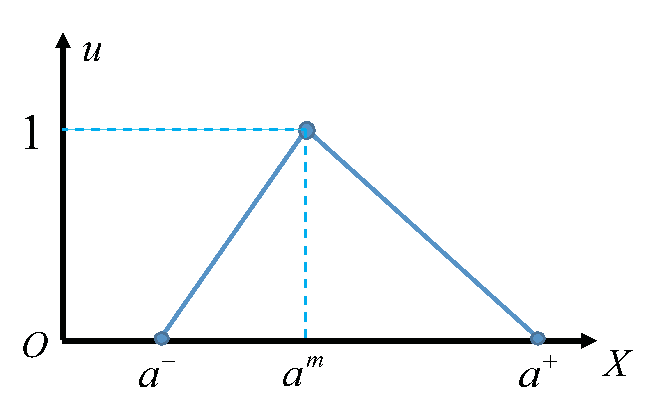
\includegraphics[width=8cm]{figures/Fig1}\\
  \caption{The triangle MF fuzzy set $\tilde{A}$}\label{fig:1}
\end{figure}

%%\begin{figure}
%%  \centering
%%  % Requires \usepackage{graphicx}
%%  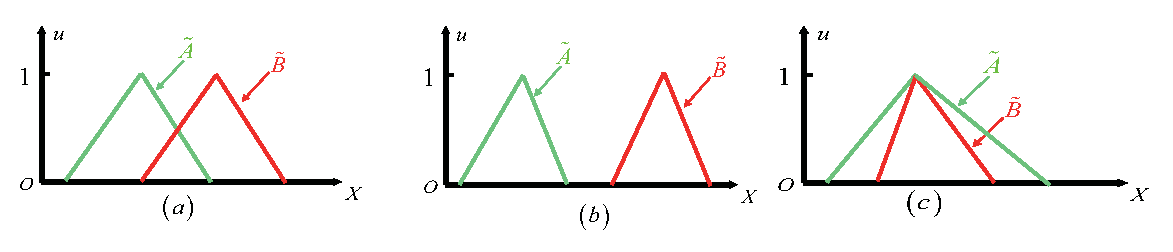
\includegraphics[width=3.2in]{figures/Fig2}\\
%%  \caption{test2}\label{fig2}
%%\end{figure}

\subsection{Definition of distance for fuzzy set valued data}

Distance is a numerical description of how far apart objects are, a distance function or metric  is a dissimilarity and triangle inequality for different datasets and plays an important role in clustering analysis. There are many distance metrics for fuzzy set data (e.g.,city-block, Euclidean, Mahalanobis, Hausdorff, Wasserstein) can be found in \citep{wang1997new, zwick1987measures, diamond1994metric, chaudhur1996metric, saha2002fuzzy, de2006adaptive, irpino2014dynamic}. However, the optimal dissimilarity metric depends on the application.

Hausdorff distance measures how far two subsets of a metric space are from each other, \cite{chaudhur1996metric} introduced a Hausdorff metric distance between fuzzy sets. Let $\tilde{A}$ and $\tilde{B}$ be two fuzzy sets, $\tilde{A_{\alpha}}$ and $\tilde{B_{\alpha}}$  be the $\alpha$  cut

%Let $\tilde{A}$,$\tilde{B}$,$\tilde{C}$ be three fuzzy sets, Then $d(\tilde{A}, \tilde{B})$ is a distance measure means if it is satisfies:

\textsl{reflexivity}: $d(\tilde{A}, \tilde{A}) = 0$, \textsl{symmetry}: $d(\tilde{A}, \tilde{B}) = d(\tilde{B}, \tilde{A})$, and  \textsl{the triangular inequality}: $d(\tilde{A}, \tilde{B}) \leq d(\tilde{A}, \tilde{C}) + d(\tilde{C}, \tilde{B})$.



\section{sec 3}
\label{sec:3}

\section{sec 4}
\label{sec:4}

\section{sec 5}
\label{sec:5}

\section{sec 6}
\label{sec:6}

%%\section{Reference}
\section*{Acknowledgments}
This research is supported in part by National Natural Science Foundation of China (Grant No.~11001019, 11471045, 41272359, 41672323) and Major scientific research projects of universities in Guangdong(2016KTSCX167).


%\begin{thebibliography}{20}
%\end{thebibliography}

\section*{References}
\bibliography{mybib}

\end{document}

\endinput
%%
%% End of file `elsarticle-template-harv.tex'.
